%
% Copyright (C) 2001 by Holger Karl,
% karl@ft.ee.tu-berlin.de
%
% file: template.tex
%
% Time-stamp: Sat Oct 06 08:29:52 2001
%
% Template fuer die Ausarbeitungen zu TKN-Seminaren
%
\documentclass[12pt,twoside,doublepage]{article}


% Hier den Namen des Teilnehmers und den Titel  der Ausarbeitung eintragen:
\newcommand{\teilnehmer}{Abdul Ahad Ayaz}
\newcommand{\ausarbeitung}{Towards Network-Aware Resource Provisioning in Kubernetes
for Fog Computing applications}


% Falls die Ausarbeitung in Deutsch erfolgt,
% die folgenden Kommentar-Zeichen '%' entfernen, andernfalls diese
 % Kommandos auskommentiert lassen:
% Languages:
% \usepackage[german]{babel}
% \usepackage[T1]{fontenc}
% \usepackage[latin1]{inputenc}
% \selectlanguage{german}

%%%%%%%%%%%%%%%%%%%%%%%%%%%
% Im restlichen Vorspann KEINE Aenderungen machen!
%%%%%%%%%%%%%%%%%%%%%%%%%%%
\usepackage{times}
\usepackage{url}

\usepackage[numbers]{natbib}

\usepackage{geometry}
\geometry{a4paper,body={5.8in,9in}}
\usepackage{titlesec}
\titleformat{\section}{\normalfont\Large\bfseries}{}{0pt}{}
% Graphics:
\usepackage{graphicx}
% aller Bilder werden im Unterverzeichnis figures gesucht:
\graphicspath{{figures/}}

% Headers:
\usepackage{fancyhdr}
% \pagestyle{fancy}
\pagestyle{fancy}
\fancyhead{}
\fancyhead[LE]{ \slshape \teilnehmer}
\fancyhead[LO]{}
\fancyhead[RE]{}
\fancyhead[RO]{ \slshape \ausarbeitung}
\fancyfoot[C]{}

\begin{document}

\title{\ausarbeitung}
\author{\teilnehmer}
\date{}
\maketitle
\thispagestyle{empty}

%%%%%%%%%%%%%%%%%%%%%%%%%%%%%%%%%%%%%%
% ab hier steht der eigentliche Text:


% Abstract gives a brief summary of the main points of a paper:
%\begin{abstract}
%  This paper gives a brief overview of the use of pigeon as a physical
%  layer underlying  the IP protocol.
%\end{abstract}

% the actual content, usually separated over a number of sections
% each section is assigned a label, in order to be able to put a
% crossreference to it

\section{Summary}
\label{sec:summary}

In recent years, with the evolution of technology, IoT devices are increasing day
by day. These IoT devices serves the mankind in different ways such as smart cites,
smart transportation, water and waste management. With this increasing number of devices,
the management and communication between these devices is one of the main issue. Fog computing
addresses this issue by connecting heterogeneous IoT devices in a network and all the processing
is done at the device level. Fog computing is the extension of cloud computing but decentralized.
\par
Fog computing is responsible for providing resouces to IoT devices for processing. Traditionally
these resources are allocated as VMs from different cloud infrastructure such as AWS, Google,
OpenStack etc. to run the applications. VMs are considered resource greedy
and require more computaional resource. Alternate is to use the Containers such as Docker[cite]
which are light-weight,requires less resources and based on micro-service archietecture. Large applications are split into
containers based on the main processes of the application. This increasing number of containers per application
required the proper monitoring for health check and resource consumption. The most commonly
used orchestrator for containers is Kubernetes[cite].
\par
Kubernetes is an open-source platform for management,deployment and scaling of containers.
Kubernetes archietecture is based on master slave model. Its consist of
one master node and multiple worker node. Worker node provides the compute power. Master node communicates
with the worker nodes using API, it is also responsible scheduling and deploying the containers
across the cluster of worker nodes. Application consisting of multiple containers are deployed
as a pod in Kubernetes. Each pod consist of only one IP address and all the underlying containers
communicate using different ports. Different pods are isolated from each other and underlaying
containers cannot communicate across pods. After receiving the pod configurations from user, master node
schedule these pods based on the resources availability on different worker nodes.

%\section{Related Work}
%\label{sec:relwork}

%The related work section could describe other work that is in some
%respects relevant for the understanding of the problem outlined in
%Section~\ref{sec:introduction}, that offer competing solutions, etc.

%All sources must be properly referenced, ideally by using the BiBTeX
%system. References can then be very conveniently made with the
%\texttt{cite} command. For example, reference
%\citenum{leuwen00:_handb_schol} discusses some of the elementary rules on
%writing scientific papers, amongst others how to correctly cite other
%documents. \citeauthor{Taylor:SIGuide:95}, e.g., describes how to
%correctly use the SI system of units and their correct typographical
%representation \citep{Taylor:SIGuide:95}.

%Since we are using the  \texttt{natbib} package in this template, it is %also convenient to
%to directly refer to the author names via the cite command -- see
%above for an example and check the natbib manual,\footnote{\url{http://www.ctan.org/tex-archive/macros/latex/contrib/natbib}}  very powerful!



%\section{Model description}
%\label{sec:model}

%After the two common sections Introduction and Related work, more
%sections with the actual content of a paper follow. The style and
%structure of such sections varies by a large degree, no general rules
%of thumb can be given.

%Such a section could, among other things, include a figure. Note that
%a figure is a so-called floating object: it is moved around the actual
%text in order to best fit on a page. This is in stark contrast to some
%GUI-based word processing tools, where the placement of figures is
%usually more associated with luck than principle.

%As figures float around, expressions like ``the following figure''
%must never be used. Instead, figures need a caption, a label, and must
%be properly referenced in the main text. An example for this concept
%is shown in Figure~\ref{fig:example}.

%\begin{figure}[htbp]
%  \begin{center}
%    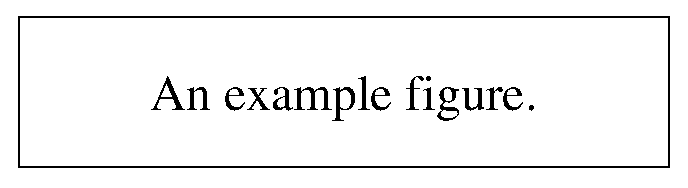
\includegraphics{example}
%    \caption{An example figure with a caption.}
%    \label{fig:example}
%  \end{center}
%\end{figure}

%In general, only vector graphics in encapsulated postscript (eps)
%format should be included in any kind of text, as this allows arbirary
%scaling, rotation etc.\ without any loss of quality. Bitmap formats
%(JPEG, GIF, \dots) should only be used if no other alternative exists
%--- basically the only case where bitmaps can be justified is when
%scanned pictures need to be included in a text, however, this should
%be avoided as hard as possible as the quality in usually not
%satisfactory. EPS files can easily be produced by most tools; for
%particular difficult cases, tools like WMF2EPS can be helpful.

%\section{Word processing \& \LaTeX}
%\label{sec:latex}

%This document has already introduced the most important constructs of
%\LaTeX. What is necessary to produce documents with \LaTeX is simple
%any normal text editor and a \LaTeX distribution. This is commonly
%installed on practically all UNIX-type systems; for Windows, an
%excellent \LaTeX exists, called MikTeX, available from
%\url{www.miktex.org}. Almost all distributions come with a large patch
%of examples and introductory material; consult your local installation
%for details.

%Lots of supplementary and background information, FAQs, etc.\ is
%available from the Comprehensive TeX Archive Network (CTAN); the
%German mirror of which is \url{www.dante.de}.

%\section{Conclusion}
%\label{sec:concl}

%At the end, there is a final section concluding and summarizing a
%paper, putting the entire work into perspective and explaining, on a
%larger level, what the consequences of this work are. Also, unexpected
%results can be discussed here, etc.


%%%%%%%%%%%%%%%%%%%%%%%%%%%%%%%%%%%%%%
% give a pointer to the bibliography information:
\bibliography{bib}

%%%%%%
% we use natbib
\bibliographystyle{plainnat}

\end{document}
